\chapter{Робинзоны}
%\corner{64}
\vepsianrose

В предыдущие два дня погода была как по заказу\mdash яркое солнце, белые кучевые облачка, красота. Но на днёвку парням погода выдалась так себе, не очень. Если с утра ещё было ничего, и они нормально приготовили завтрак, то~потом налетел шквал, с юга начала сгущаться дождевая облачность, краски дня пожухли, всё стало серым, мрачным.

После традиционной каши чемпионов с утра все развалились на стульчиках под тентом у стола, состояние было ленивым. Островные Робинзоны выспались, отдохнули. Киря внезапно развёл деятельность:

\diagdash Шурик, мне нужна вторая чалка!

\diagdash На кой она тебе?

\diagdash Ну мы ж пороги завтра берём, а у меня только носовая чалка, кормовой нету!

\diagdash Кирь, у меня тоже только носовая чалка, а кормовой нету и не было отродяся.

\diagdash А вот когда я ходил по Керети$\ldots$

\diagdash Зачем она нужна, кормовая?

\diagdash Да мало ли что!\mdash Замполит что\sdash то начал разводить нервы.\mdash Смотри, это может пойти на чалку?\mdash он достал моток белой синтетической ленты.

\diagdash Ё-моё! Нафига ты это тащишь с собой?\mdash Адмирал всегда ратовал за уменьшение количества вещей, без которых можно обойтись.

\diagdash Ну, ты говорил, что вещи будем вязать к каркасу$\ldots$

Адмирал вспомнил, что действительно были такие разговоры:

\diagdash Да, говорил, но судя по тому, как мы вчера всё прошли, по\sdash моему, это лишнее. Кстати, из этой ленты можно сплести чалку, раз ты так хочешь.

\diagdash Сплести?!\mdash переспросили Серёга с Кирей.

\diagdash Ну да, а что? Как косичку, из трёх лент. Тащи сюда свой моток!

Они нашли старый ржавый гвоздь, вбитый в сосну поблизости\mdash остатки чьей\sdash то старой стоянки\mdash и, вколотив его топором в сосну получше, привязали к нему три ленты:

\diagdash Так, ну теперь плетём.\mdash Адмирал сел на складной стульчик и начал пробовать.\mdash Руслан, подсоби!

Тот тоже взял раскладной стульчик, сел рядом, и~они в~четыре руки начали плести\mdash сначала просто переплетали ленты, поджимая получающуюся косичку, но~потом поняли, что по мере плетения <<хвост>> этой косы в~бухте приходится разматывать в обратную сторону, что было жутко неудобно. Поэтому они решили сделать три <<катушки>> с лентой, намотав её на палочки, чтобы получились такие большие шпули. После того, как три шпули были готовы, дело пошло гораздо веселее, ничего не~запутывалось:

\diagdash Перехватывай.\mdash Адмирал передавал одну шпулю Руслану, перекрещивая ленты в плетении.\mdash И давай сюда обратно!

\diagdash Ручной ткацкий станок!\mdash Руслану было по приколу поучаствовать в затее.

\diagdash Пацаны, у вас клёво получается!\mdash Замполит завороженно стоял рядом и наблюдал как парни плетут уже третий метр чалки. Руки их так и сверкали, перекрещиваясь и меняясь перехватом шпуль.\mdash Быстро у вас получается!

\diagdash Хочешь сам?

\diagdash Не-не-не, я смотрю вы такие профессионалы, что куда уж мне!\mdash отшутился Замполит.

На плетение чалки ушло часа два, а то и больше\mdash когда ребята закончили, погодка нахмурилась\mdash и~если с утра было достаточно тепло и Адмирал расхаживал с голым торсом, то сейчас ему пришлось утеплиться в~штормовку.

\diagdash Так, вяжи узел на конце, давай попробуем канат на~прочность!\mdash Адмирал докончил плести, встал, размялся и растянул их творение.

\diagdash Да вроде не рвётся!\mdash заключил Киря, наблюдая за~тем, как Адмирал оттягивает собой новоиспечённый канат.

\diagdash Пользуйся!\mdash Адмирал сбухтил чалку и кинул её Замполиту\mdash тот пошёл вязать к байде.

%\begin{wrapfigure}[15]{l}{0.6\textwidth}
\begin{figure}[h]
	\centering
	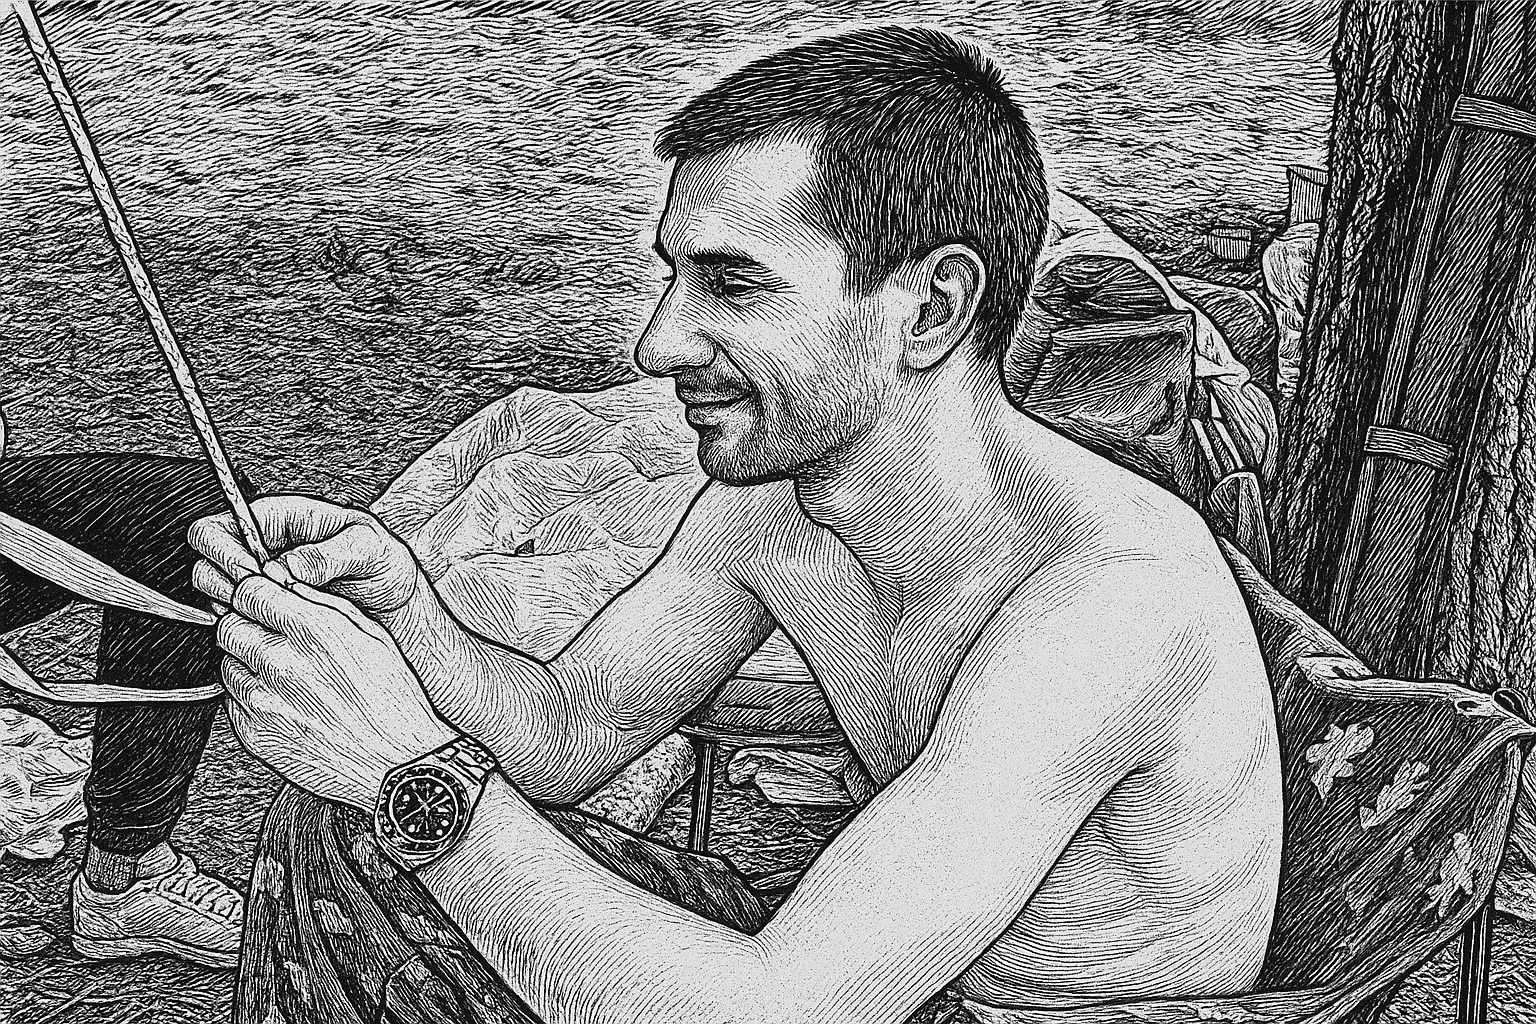
\includegraphics[width=1.0\textwidth]{28_chalka}
	\caption{\small\textit{...из этой ленты можно сплести чалку...}}
\end{figure}
%\end{wrapfigure}
После того, как немного развлеклись с плетением, все вновь расселись под тентом у стола:

\diagdash А что у нас со связью всё таки?\mdash Паша сидел у~стола и пил чаёк с конфетами.

\diagdash О! А надо знаете что сделать? Надо взять ту же ленту, из которой чалку плели, обвязать какой\sdash нить камешек, перекинуть это дело через ветку сосны, да хотя бы вон той,\mdash Адмирал показал на росшую рядом с их поляной высокую красивую сосну с раскидистыми ветками,\mdash и поднять туда наверх телефон, скажем, в обрезке пластиковой бутылки!

\diagdash А что, идея! Чей телефон будем поднимать? Чур,~не~мой!\mdash ответил Паша.

\diagdash Ну чей, чей. Знамо, чей\mdash замполитовский, больше\sdash то~чей?\mdash заключил Адмирал.

\diagdash Чойта?\mdash отозвался тот.

\diagdash Ну как <<чойта>>? Такая вот доля твоя!\mdash иронизировал Адмирал.\mdash Да лан, расслабься! На самом деле только у тебя в Нёлгомозере ловило связь, так что выбор очевиден.

\diagdash Блин, и не поспоришь. Ну давай$\ldots$

Адмирал обвязал камешек лентой и перебросил через высокую ветку. Потом связал ленту в кольцо и подвязал к ней обрезок пластиковой бутылки, которой пришлось пожертвовать. Замполит скрепя сердце подошёл и положил в приспособу свой мобильник:

\diagdash Поехали!

Телефон медленно пополз вверх. Команда смотрела за~всем этим действом из\sdash под тента.

\diagdash Шурик, хар{\'о}ш, хар{\'о}ш!!!\mdash Киря переживал.

\diagdash Не очкуй, аллес унтер контролле!\mdash тот поднял телефон наверх до предела, они подождали пару минут, спустили обратно.

\diagdash Ну и нифига!\mdash раздосадованно сказал Замполит.

\diagdash Как нифига???

\diagdash Ну так!!! Не грузится страница\mdash <<палочек>> связи даже нет, о чём разговор?

\diagdash Да ёпрст!

Они промучились ещё минут пятнадцать, но ничего не~вышло:

\diagdash Надо бы там, наверху когда телефон, нажать кнопку <<обновить страницу>>!\mdash догнал Замполит.\mdash Без этого ничего не получится.

\diagdash Умный, блин! Если бы можно было туда залезть по~голому стволу, то и верёвка эта нафиг не нужна!

\diagdash О, а ещё можно сплести верёвочную лестницу$\ldots$

\diagdash Я с вас угораю!\mdash ржал под тентом Паша.

\diagdash Ладно, версия с сосной провалилась, ещё варианты?\mdash вопрошал Адмирал.

\diagdash Хм-м-м! Ну, вчера была версия, что надо идти на~мыс пытаться там ловить связь, наскока я помню.\mdash сказал Серёга.\mdash Пошли, Кирь, сходим с тобой наверно?

%\diagdash Походу да, придётся$\ldots$ Во всяком случае, это самое разумное.
\diagdash Мне кажется это самое разумное.

Времени было уже к часу дня, когда Киря с~Серёгой собрались в~поход по острову. Погода окончательно нахмурилась, закапал редкий дождик. Остальная команда сидела, блаженно развалившись на стульчиках под тентом:

\diagdash Так, Робинзоны, давайте! Я в вас верю! Без описания маршрута не возвращайтесь!\mdash напутствовал Адмирал.

\diagdash Приободрил так приободрил!\mdash те взяли с собой топорик на всякий случай и пошли. Паша и Руслан с~Адмиралом остались у костра и продолжили чаёвничать:

\diagdash Что будем делать без описания маршрута?\mdash спросил Руслан, когда ушедшие ребята скрылись в лесу за пригорком.

\diagdash Ну как что, идти маршрут дальше, а что ещё? Не~сниматься же позорно из\sdash за этого? У нас всего\sdash навсего вторая категория, не~пятая.\mdash напомнил Адмирал.\mdash Вторая ещё прощает ошибки прохождения$\ldots$

\diagdash Тем более мы всегда так ходим\mdash этот,\mdash Пашка махнул кружкой в сторону Адмирала,\mdash прочитает чё нить про маршрут и нихрена никому ничё не расскажет, а мы потом вляпываемся!

\diagdash Да лан тебе, разошёлся прям! Когда такое было?\mdash оправдывался Адмирал.\mdash Ну, может пару раз и то некритично!\mdash покопавшись в воспоминаниях, ответил он.

\diagdash Ну, на Песи с обносами и завалами$\ldots$\mdash Пашка вспомнил их поход пятилетней давности.

\diagdash Ну и обнесли, не умерли?\mdash напомнил Адмирал.

\diagdash Это да$\ldots$\mdash согласился тот.\mdash Потом ещё чёт было такое, не помню уже$\ldots$ А! Сливчик на Песи был типа~порожка.

\diagdash Всё некритично\mdash все живы, здоровы, снарягу не~потеряли, сами не убились, значит порядок!\mdash заключил Адмирал и прихлебнул.

\diagdash Это оно раньше так удачно всё было$\ldots$ А вот завтра как будет\mdash хрен его знает!\mdash Паша тоже прихлебнул.\mdash C ним,\mdash опять показав на Адмирала,\mdash не пропадёшь, да\sdash а\sdash а.\mdash сказал он, немного стращая Руслана.

\diagdash Я, между прочим, всегда всем рассылаю описание маршрута, просто никто не читает же.

\diagdash Ну, это да$\ldots$

\diagdash Киря только что\sdash то меня расстраивает.\mdash поделился своими опасениями с экипажем Адмирал.\mdash Не захотел порог идти вчера, руками тащил. А что завтра будет? Завтра настоящие, всамделишние пороги пойдут.

\diagdash Тогда вчера что было? Не всамделишние?\mdash удивился Руслан.

\diagdash То была разминка, они на топокарте как пороги\sdash то даже не обозначены$\ldots$

\vspace{0.5cm}
$\ldots$Робинзоны вернулись через час, не меньше:

\diagdash Так, ну что\sdash то получилось загрузить!!!\mdash обрадовал команду Замполит.

\diagdash Класс! Докуда дошли?\mdash спросил Адмирал.

\diagdash Черноволосую видели?\mdash посыпались вопросы.

\diagdash Да практически до той стоянки на мысу дошли, которую видели вчера. У них лодка под мотором.\mdash отвечал Серёга,\mdash Мужика какого\sdash то видели, да и всё.

\diagdash А валькирию?

\diagdash И след простыл$\ldots$\mdash вздохнули парни.

\diagdash Может её и не было?

\diagdash ???

\diagdash Ну, например, нам привиделось.

\diagdash Алё, алё! Недели похода ещё нет, а вам уже мерещится что ли?

%\renewcommand*{\thefootnote}{\arabic{footnote}}
\renewcommand*{\thefootnote}{\fnsymbol{footnote}}
\setcounter{footnote}{0}

\diagdash А что? Ф\'ата\sdash морг\'ана\footnote{Ф\'ата\sdash морг\'ана (итал. Fata Morgana)\mdash сложная и редко встречающаяся форма миража.}, слыхал про такое?

\diagdash Ой, я с вас угораю!\mdash поржал над ними Паша.

\diagdash Ладно, по делу давайте. Описание есть\mdash уже хорошо. А те деятели, стало быть, сюда против течения дошли? На~моторке\sdash то.\mdash предположил Адмирал.

\diagdash Почему? Может и с верховьев Суны?\mdash размышлял вслух Серёга.

\diagdash Не-е-е, с верховьев навряд ли, там же воды меньше, пороги жёстче. А они на моторке. Это с деревни, сто процентов.\mdash предположил Паша.%предложил народу наиболее убедительный вариант Паша.

\diagdash Да ну не факт! Подними в порогах движок и всё! Мы~же~не~знаем, что там выше по Суне.\mdash пошли толки.

\diagdash Забейте, главное теперь у нас есть описание порогов! Давайте читать, Робинзоны, ёпрст!\mdash Адмирал приободрился.

\diagdash Так насухо как\sdash то$\ldots$\mdash предложил Паша.

\diagdash А у меня винишко есть$\ldots$\mdash сказал робко Руслан.\mdash Спецом на днёвочку.

\diagdash Ё-моё, ты в стекле тащил?\mdash Адмирал немного негодовал.

\diagdash Ага!$\ldots$\mdash сознался тот.

\diagdash Тащи сюды! Уменьшим вес байды перед порогами!\mdash однозначно заключили все.

Погодка, тем временем, была совсем не винной\mdash зарядил ливень, да такой, что в ослабший за ночь тент над~столом стала набираться вода.

\diagdash Шурик, надо бы слить воду\sdash то$\ldots$\mdash Замполит посмотрел вверх на тент.

\diagdash Надо! Надо под дождь идти. Иди?\mdash Паша разливал всем желающим красненького.

%\begin{wrapfigure}[15]{l}{0.6\textwidth}
\begin{figure}[h]
	\centering
	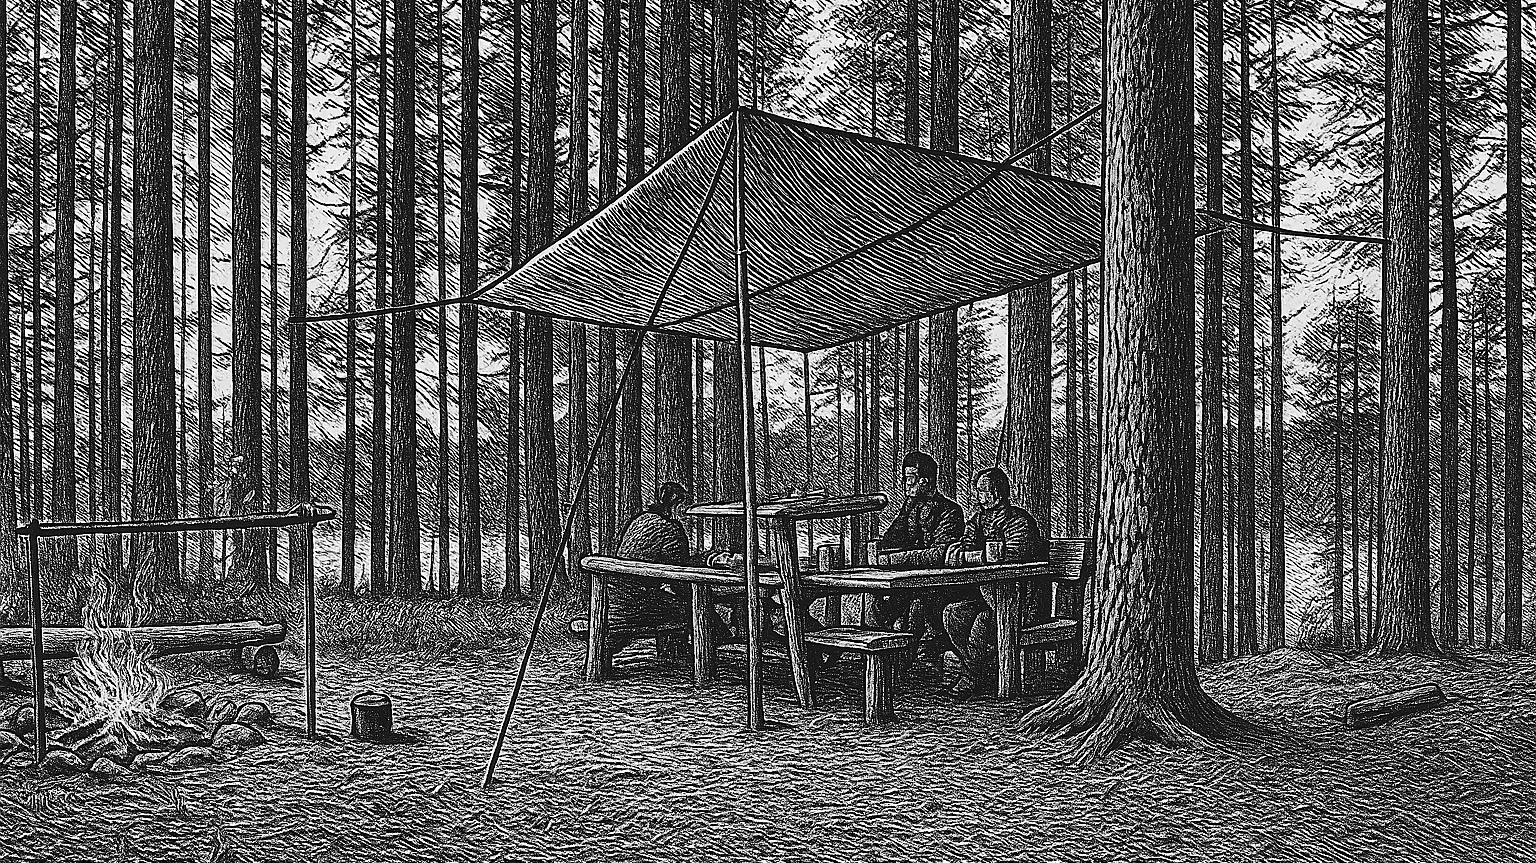
\includegraphics[width=1.0\textwidth]{29_tent}
	\caption{\small\textit{...в ослабший за ночь тент над~столом стала набираться вода...}}
\end{figure}
%\end{wrapfigure}

\diagdash Ы-ы-ы!

\diagdash Пофиг, потом!

\diagdash Ы-ы-ы! Разливай, да подставляй, не зевай!

Дождь барабанил крупными каплями по тенту, сплавщики сидели под ним, укутавшись в штормовки, и~читали описание порогов, закусывая:

\renewcommand*{\thefootnote}{\arabic{footnote}}
%\renewcommand*{\thefootnote}{\fnsymbol{footnote}}
\setcounter{footnote}{0}
\diagdash Так! <<Первый порог,\mdash читал Замполит с~телефона,\mdash Уйтуженкоски. Длина его около одного километра. Русло реки прямое и широкое. Осмотр слева. На входе под левым берегом шивера\footnote{Относительно мелководный участок реки с беспорядочно расположенными в русле подводными и выступающими из воды камнями и быстрым течением.} с бурным течением. Далее надо переходить под правый берег\footnote{Здесь и далее описание порогов из~\cite{Шилов}.}>>. Охренеть!\mdash прокомментировал он и~продолжил:\mdash <<В низкую воду в~струе появляются два опасных обливняка, хорошо заметных по пенным гребням за~ними>>. Сечёте, парни?

Адмирал сходил к палатке, достал командирский планшет, открыл бумажную заламинированную карту, ту~самую, что ламинировали у Замполита. Он оценил ещё раз предварительные стратегии прохождения маршрута в~целом и заключил, что хорошо бы завтра дойти до устья Черанги\mdash там, судя по описаниям, было хорошее стояночное место.

\diagdash Ну понятно\mdash там сказано идти под левым берегом, потом по ходу прохождения порога переходить к центру и~под правый. Там река как раз правый поворот делает.\mdash заключил Адмирал.

\diagdash Это как?\mdash Серёга не понял.

\diagdash Там простор будет$\ldots$ Это вчера\mdash речка\sdash переплюйка десять метров шириной. А там,\mdash Адмирал уточнил по~карте,\mdash написано все 50, а то и 100 метров местами.

\diagdash !!!

\diagdash Да не очкуйте, это всего лишь вторая категория! Читай дальше, Кирь.

%\renewcommand*{\thefootnote}{\arabic{footnote}}
\renewcommand*{\thefootnote}{\fnsymbol{footnote}}
\setcounter{footnote}{0}
\diagdash Ага! Гм, так$\ldots$ <<После плёса\footnote{Широкое водное пространство или часть водоёма, отличающаяся большей (по сравнению с соседними водными участками) глубиной.} идёт порог Шильмятойкоски>>$\ldots$

\diagdash Стопэ! У меня на карте ещё два безымянных порога перед Шильмятойкоски.\mdash встрял Адмирал.

\diagdash Эм$\ldots$ Шурик, а про них не написано ничего!\mdash оторвался Замполит от телефона.

Повисла короткая немая пауза, которую прервал Паша:

\diagdash Кому подлить? Гуляй, рванина! Может больше не~придётся пить вино и есть хлеб!

\diagdash Ы-ы-ы,\mdash заржал Адмирал,\mdash вы угораете? Давай дальше читай. Если нет ничё про те пороги, значит они ерундовые.

\diagdash То есть такие ерундовые, как вчера?\mdash уточнил Серёга.

\diagdash Ага!

\diagdash Ну тогда я спокоен, ха-ха!\mdash слегка истерически засмеялся тот.

Киря уткнулся в телефон, продолжив:

%\renewcommand*{\thefootnote}{\arabic{footnote}}
\renewcommand*{\thefootnote}{\fnsymbol{footnote}}
\setcounter{footnote}{0}
\diagdash <<$\ldots$Шильмятойкоски, где после поворота есть мощная бочка\footnote{Обратное течение, возникающее за мощным крутым сливом после препятствия в русле. Опасно тем, что удерживает плавсредство, не давая выбраться.} за плитой>>.\mdash Шурик, какого хрена это вторая категория?

\diagdash Чё ты у меня спрашиваешь? Ты так угораешь, как будто я перед походом не рассылал всем описание маршрута. Те, кто проходил\mdash им виднее, наверно, насчёт категории? 

\diagdash После них такие таблички бронзовые на скалах, случаем, не остались с именами и годами жизни?

\diagdash Завтра увидишь, ы-ы-ы!\mdash Адмирал поднялся и~решил всё таки слить дождевую воду, набравшуюся в~провисший тент.\mdash Ты читай\sdash читай давай!\mdash а сам, накинув капюшон штормовки, вышел под дождик и подтянул оттяжки тента карабинами, слив воду, после чего вновь уселся назад к~команде за стол.

\diagdash Та-а-ак, дальше чё тут$\ldots$ <<Ковеланлиете\sdash Коски\mdash длина около двухсот метров, на входе есть пологий слив в~скальном сужении, затем крутой левый поворот с грядой камней слева>>$\ldots$

\diagdash Ну никакой жести же?

\diagdash Далее$\ldots$ <<Шестисотметровый перекат с тремя поворотами в русле и порог Леполису\mdash крутая 150\sdash метровая шивера>>$\ldots$

\diagdash Кирь, у меня перед Леполису не обозначено ничего по карте. Я думаю прям всё\sdash то читать не обязательно, сейчас ничего не запомнишь. Перед каждым порогом, я полагаю, имеет смысл читать, чтобы прям непосредственно перед прохождением.\mdash заметил Адмирал.

\diagdash А как ты узнаешь когда порог?\mdash спросил Серёга, прихлебнув из кружечки.

\diagdash Ну, во\sdash первых, они, те которые на карте и в описании есть, отмечены у меня в навигаторе, а навигатор у меня на~шее висит и пищит при приближении к путевой точке. Во\sdash вторых, ты по звуку, шуму воды, издалека услышишь, уж~поверь\mdash заверил команду Адмирал.

\diagdash Ладно, успокоил$\ldots$

\vspace{0.5cm}
$\ldots$Дождик кончился, но погода не улучшалась, висела низкая сплошная облачность. Лес после дождя был мокрым. Парни решили подзаготовить дров на вечер и завтрашнее утро и разбрелись по лесу. Обильно смоченный дождём мшаник под ногами был мягким, как воздушное одеяло. Адмирал решил пройти чуть подальше от лагеря. Он шёл широкими шагами, стараясь не намочить кеды, по~своему любимому типу леса\mdash сосновому, без подлеска, с~обильным зелёным и белёсым мхом. Вскоре он заприметил две тонкие длинные сухие подгнившие снизу сосны. Завалив два сушняка голыми руками, он потащил их в лагерь, волоча за~собой. Парни тоже притащили к костру кто чего. Свалили запасец дров неподалёку и снова собрались под тентом:

\diagdash Шу-у-урик, а спасжилеты? Ты их испытывал?\mdash поинтересовался Серёга.

\diagdash Не-а! А зачем?\mdash Адмирал потянулся.\mdash Жилеты как жилеты. Они же ненадувные\mdash надел и всё.

\diagdash Я бы пошёл попробовал$\ldots$ Заранее, так скажем.

\diagdash Парни, ну чё вы очканули\sdash то? То, что вчера вляпались\mdash да, мой косяк, что я забыл описание, а~связи не было. Но выжили же, потерь среди личного состава и~имущества нет! А боевой дух мы щас активно укрепляем!\mdash Адмирал повернулся и обратился к Паше:\mdash Плесни\sdash ка?\mdash тот ливанул ему красненького. Отпив, Адмирал продолжил,\mdash Если бы вчера заранее знали о~том пороге, спорим не так бы всё было?

\diagdash Слишком много <<бы>>, но предположим$\ldots$

\diagdash Во-о-от именно!\mdash продолжил Адмирал.\mdash А~теперь у нас есть описание, и мы морально готовы. У нас есть ёмкости непотопляемости в байдах\mdash по 6 штук на~каждую, фартуки, юбки, спасжилеты, радиосвязь! Мы не~просто подготовлены, а~сверхподготовлены. Оба~капитана\mdash на~опыте, так что давайте, не~очкуйте! Спасжилеты\mdash это вообще крайний случай, я считаю. То~есть вариант, когда они понадобятся\mdash это вообще~жопа. Подразумевается, что ты должен выпасть, выплыть из~байдарки и~существовать отдельно от неё, чтобы тебе понадобился спас. А,~я~напоминаю, в байдарке все наши вещи, жратва и~прочее\mdash за байдарку боремся до~последнего, в~случае чего. Вы себя накрутили на~ровном~месте!

\diagdash Ты просто не килялся в порогах$\ldots$\mdash мрачно вставил Замполит.\mdash А вот я на Керети$\ldots$

\diagdash Кирь, Кереть категорией выше. Думаешь категории просто так дают? Ещё раз, парни, вариант когда вы оказались в воде на пороге\mdash это, как говорят, <<максимальная проектная авария>>, то есть когда ты уже не проходишь маршрут, а борешься за живучесть. При оверкиле утонуть вам не даст спас, а далее, не бросая весла, надо держаться за~байду. Тонуть она не должна, теоретически\mdash в гермах всё равно есть воздух, как и в ёмкостях непотопляемости, это я так пафосно наши пустые 5\sdash литровые бутылки называю. Вот~и~всё.\mdash Адмирал, толкнув речь, откинулся в стульчике довольный собой и жадно осушил кружечку.

\diagdash Ух! Ну ладно, убедил!\mdash речь не прошла даром.

\diagdash А, и это, щас <<морковку>> потренируемся кидать!\mdash после дождя в лесу было мокровато, но потренироваться в~бросании надо было, решил Адмирал.

\diagdash <<Морковка>>\mdash это что?\mdash уточнил Руслан.

\diagdash Это спасконец Александрова.\mdash Адмирал уже сгонял к байдарке и притащил его.\mdash Вот, гляди\mdash в оранжевом мешочке это действительно похоже на морковку. Давайте, каждый раза по два кинет.\mdash сказал он и первым, широко размахнувшись из\sdash за спины, метнул мешочек вперёд. Оранжевая упаковка улетела далеко за поляну, жёлтый трос стремительно размотался в полёте.\mdash Примерно вот так это и выглядит. Бросать надо чуть выше по течению, поскольку <<морковку>> начнёт сносить. Прицеливаться надо хорошенько, потому что повтор броска возможен только после того, как смотаешь опять трос в мешочек, а это время.

Он смотал трос, заново бросил и, опять смотав, передал следующему:

\diagdash Тренируйтесь, парни! Каждый по 2\thinspace\nobreakdash---\thinspace 3 раза пусть бросит, надо чтобы вы почувствовали как она летит, вдруг понадобится.

Парни по очереди, уже без прежней доли пессимизма, со~смешками, пошли кидать <<морковку>>, а Адмирал подбросил дров в костёр:

\diagdash Борща что ли наварить? Хм-м-м$\ldots$ Не, попозже маленько.\mdash и~решил искупаться в озере.

Команда, накидавшись <<морковку>>, свернула её, после чего настал черёд спасжилетов:

\diagdash Шу-у-урик, я пойду попробую спас на воде.\mdash больше всех переживал Серёга. 

\diagdash Давай! Я не против. Я купаться туда пойду ща.\mdash Адмирал вытащил банные принадлежности и пошёл купаться нагишом, как он любил делать это в сплавах.

\diagdash Пацаны, да вы моржи нафиг!\mdash Кире купаться лишний раз не хотелось. 

\diagdash Ух-х-х! Не так и холодно!!!\mdash доносились с~берега возгласы Адмирала.

Погода стояла после полудня пасмурная, свинцовое низкое небо было не слишком приветливым, днёвка проходила достаточно лениво. Адмирал искупался, а Серёга, который плохо плавал и~более всех, надо полагать, переживал за мокрую часть программы, \begin{wrapfigure}[10]{r}{0.55\textwidth}
	%\begin{figure}[h]
	\centering
	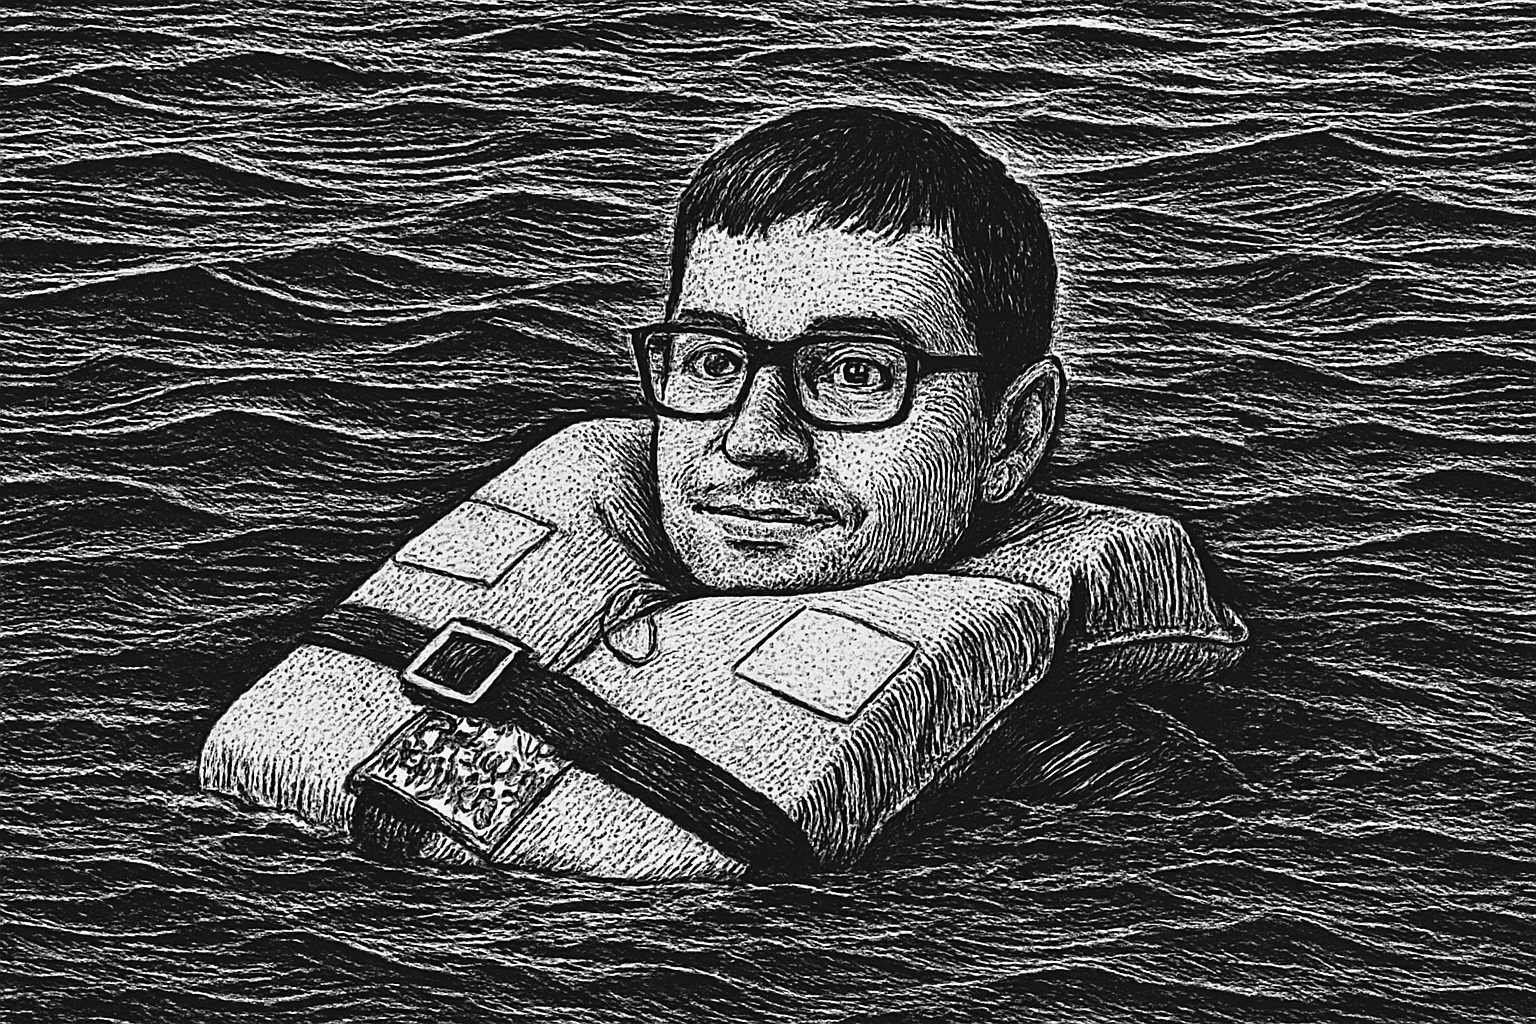
\includegraphics[width=0.5\textwidth]{30_lifejacket}
	\caption{\small\textit{...испытал свой спасжилет...}}
	%\end{figure}
\end{wrapfigure}испытал свой спасжилет и~успокоился. Руслан с~Пашей тусили под тентом, приканчивая красненькое:


\diagdash С бутылками что делать будем с пустыми? Не круто после себя стекло оставлять. Эх, молодо\sdash зелено, кто ж в~стекле с собой тащит?\mdash Паша разлил последнее.

\diagdash В костёр положи и прикрой сверху дровами, чтобы не~отскочили осколки, если что. Помнишь, мы так делали, когда сплавлялись по Чагодоще? Там переплавили вообще в~какой\sdash то мелкий кусочек, по\sdash моему.\mdash предложил Адмирал Паше, идя к палатке после купания.\mdash Водичка\mdash кайф, мужики! Подкиньте дров, надо обсохнуть!

\diagdash Не, там ваще ничего от тех бутылок не осталось! Мы ворошили потом угли и не нашли стекла, приколи?\mdash вспомнил Серёга былое.

\diagdash Да\sdash а\sdash а, это был <<арктический>> поход '19 года, помните? Странно, что по Чагодоще айсберги не плавали.

\diagdash Такое забудешь, пожалуй! Весь поход в свитере!

\diagdash Ы-ы-ы! Зато впечатлений$\ldots$

Адмирал, взбодрившись купанием, обсох у огня, утеплился и принялся за готовку:

\diagdash Давайте борща замутим!!!

\diagdash Офигеть, я тут лучше чем дома питаюсь!\mdash сказал Руслан.

Адмирал не поверил своим ушам и повернулся к тому:

\diagdash Да ладно?!

\diagdash Ну вот так. Я ж один живу.

\diagdash А-а-а! Все остальные\sdash то у нас женатики. Подкаблучники! Да, Замполит?\mdash Шурик не преминул подколоть Кирю.

\diagdash Ой, Шурик, кто б говорил!!!\mdash отозвался тот.

\diagdash Ы-ы-ы!!! Ладно, Руслан, дай сковородочку, давай забацаем офигенскую зажарку для борща, а?\mdash и Адмирал обжарил почищенную и нашинкованную полосками свеклу, а потом и морковь с луком. Он любил готовить на костре, потому как на костре что ни приготовь, почему\sdash то всё вкусно получается. Особенно вечером после перехода длинного\mdash всё сметается просто в мгновенье ока.

Пока Адмирал священнодействовал, колдуя над~борщом, Паша, как всегда, подсуетился с нарезкой хлебушка, сала, лука, апельсина. Стол ломился от закуски. Адмирал покопался в герме, вытащил банку паштета и~наделал бутеры. На второе он сообразил булгур с~сушёными томатами и тушёнкой. Словом, баловал команду, ибо ну~а~для чего они ещё здесь? Отдых душой и телом. Когда всё было готово, он~позвал~всех:

\diagdash Ку-у-ушать! Тару сюды!

Все стали подходить с мисками, тарелками, подкотельниками, кто из чего ел. Он раздал всем половником из котелка, а после ребята расселись по~стульчикам, креслам и брёвнам у костра:

\diagdash Кайф, мужики! Хочу, чтоб это длилось вечно!\mdash Адмирал вдыхал аромат борща.

\diagdash Вечно если\mdash надоест!\mdash справедливо заметил Серёга.

\diagdash Борщ ваще класс, мне не надоест!\mdash Руслан наворачивал с хлебом.

%\noindent
%\begin{minipage}{0.48\textwidth}
%	\setlength{\parindent}{1.0cm}  % Включаем красную строку
%	
%	\indent \diagdash Так, давайте, парни, под горячее! Паш, разливай там, что~ли?\mdash обратился к тому Адмирал.
%	
%	\diagdash Таки уже!\mdash тот был наготове.\mdash И сальцо, и лучок, всё в наилучшем виде!
%	
%	Адмирал оглядел свою бравую команду, поднял кружку и заорал:
%	
%	\diagdash {\Large SKÅ-Å-ÅL!!!}
%\end{minipage}\hfill
%\begin{minipage}{0.5\textwidth}
%	\centering
%	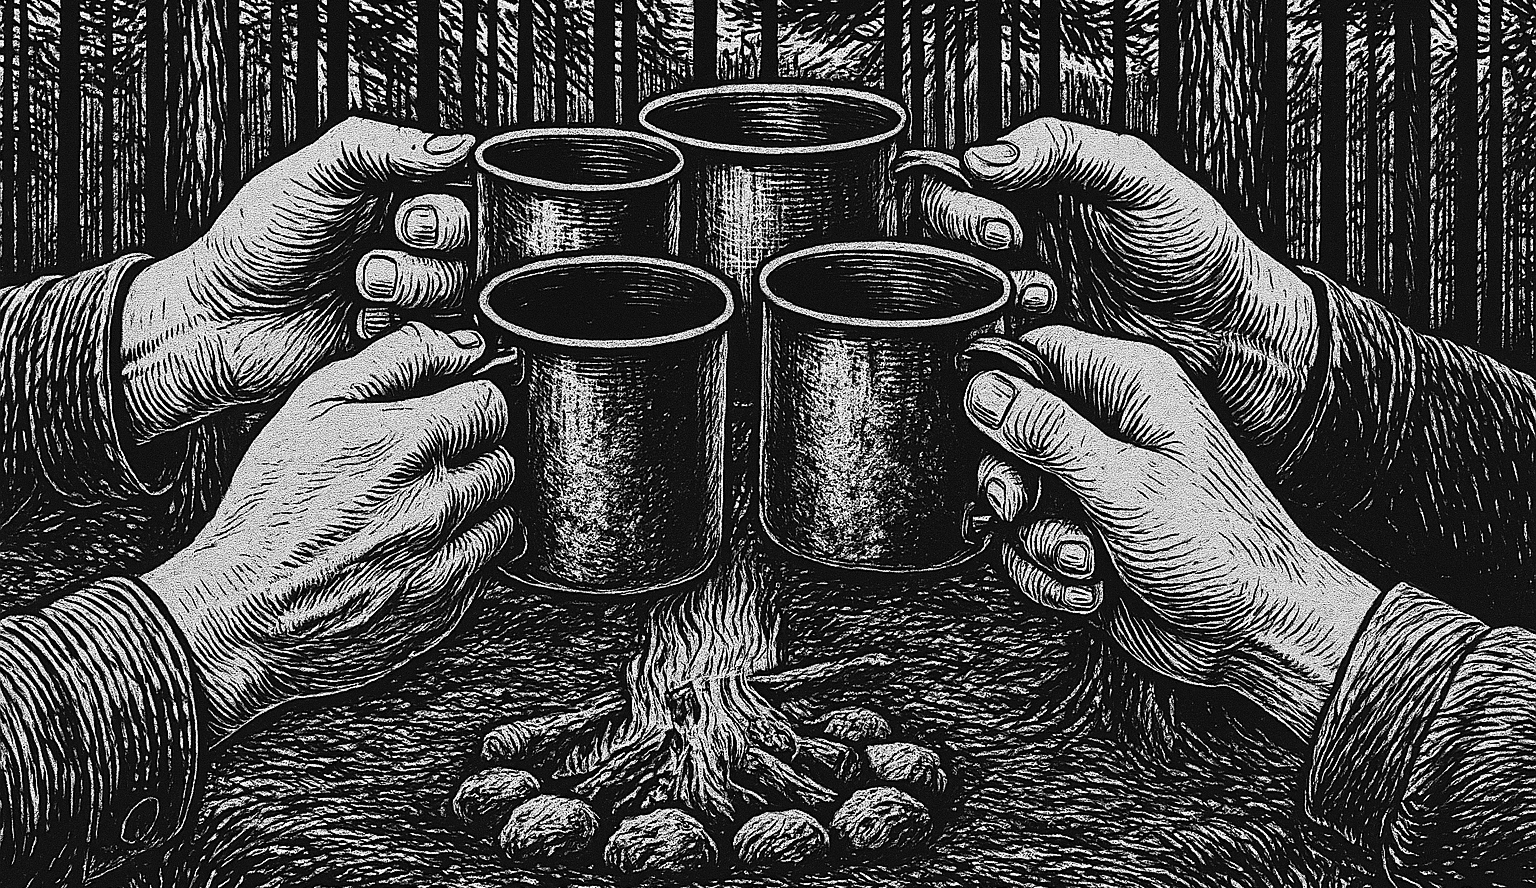
\includegraphics[width=\linewidth]{10_2_new}
%	
%	{\small\textit{...SKÅ-Å-ÅL!!!...}}
%\end{minipage}

%\begin{wrapfigure}[10]{l}{0.62\textwidth}
%%\begin{figure}[h]
%	\centering
%	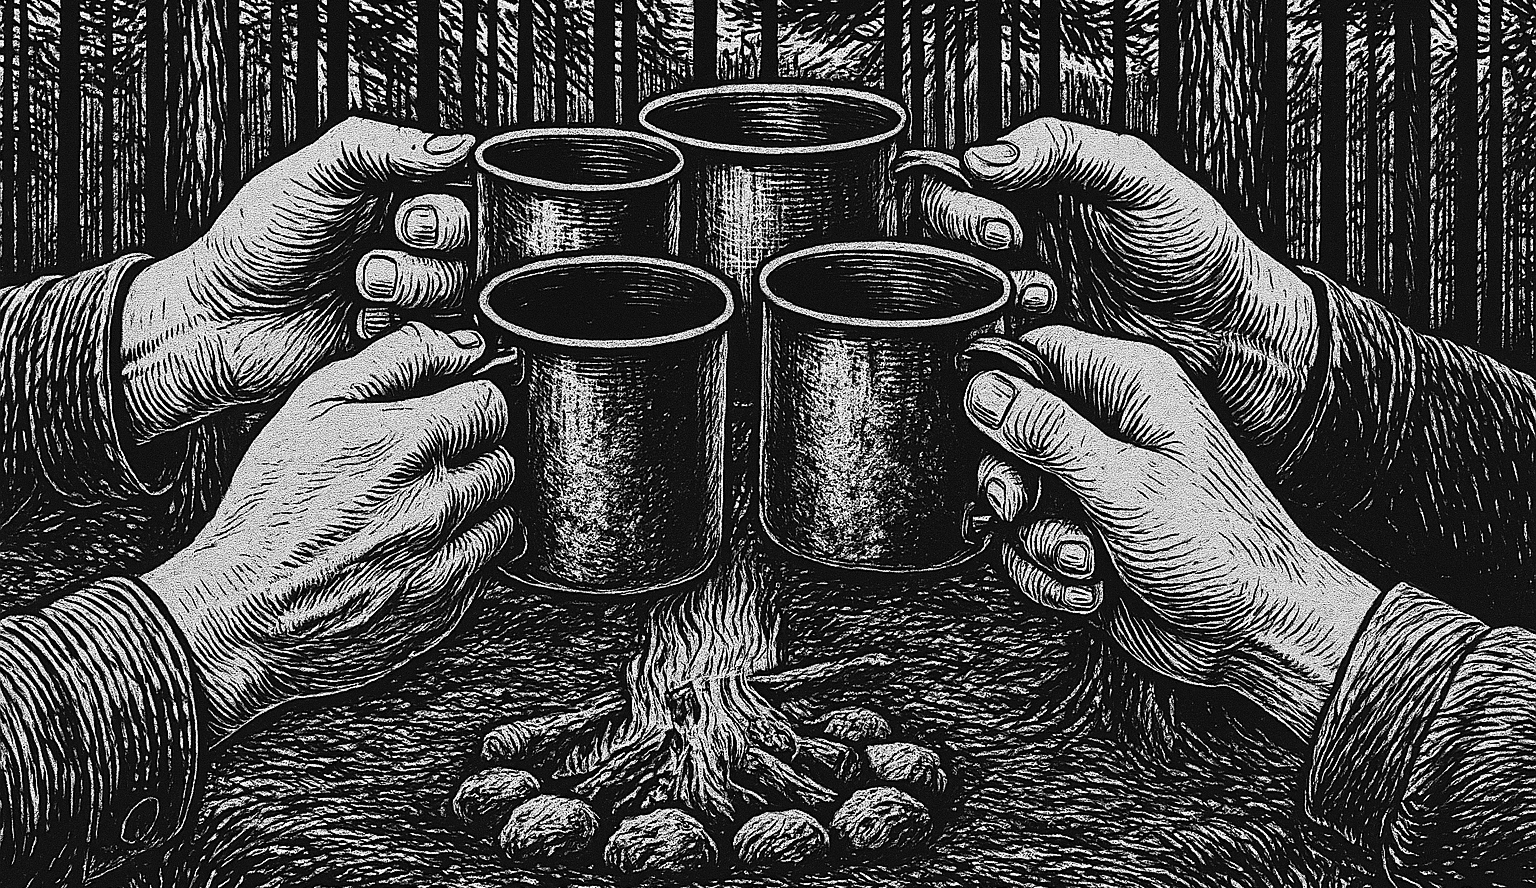
\includegraphics[width=0.62\textwidth]{10_2_new}
%	\caption{\small\textit{...поднялся лес рук...}}
%%\end{figure}
%\end{wrapfigure}

\diagdash Так, давайте, парни, под горячее! Паш, разливай там, что~ли?\mdash обратился к~тому Адмирал.

\diagdash Таки уже!\mdash тот был наготове.\mdash И~сальцо, и~лучок, всё давно готово в~наилучшем виде!

Адмирал оглядел свою бравую команду, первым поднял кружку и бешено заорал:

\diagdash {\Large SKÅ-Å-ÅL!!!}

\diagdash {\Large SKÅ-Å-ÅL!!!}\mdash яростно подхватила команда, поднялся лес рук.

\diagdash Кампа-а-ай!\mdash тоненько передразнил их Пашка.

\diagdash Фу ты, ну ты!

%\diagdash Ы-ы-ы!

Сытые довольные сплавщики блаженствовали у костра, но тут опять закапал дождик. Пришлось переместиться под~тент.
Остаток вечера прошёл у~них в подогретых замполитовых переживаниях по поводу порогов и~не~менее подогретых~адмиральских увещеваниях, что они все зря очкуют.
Спать все завалились не слишком поздно\mdash Адмирал дал отбой пораньше, надо было выспаться перед завтрашним штурмом порогов.

\begin{center}
	\psvectorian[scale=0.4]{88} % Красивый вензелёк :)
\end{center}
